\documentclass[Main.tex]{subfiles} 
\begin{document}

\subsection{Oversigt over arkitektursignifikante Use Cases}
I dette afsnit er de enkelte Use Cases pr�senteret. Alle Use Casene bliver pr�senteret, da de alle er centrale for systemets fuktionalitet, samtidig med at systemet kun best�r af fem Use Cases. 
\\
Use Casene i systemet er f�lgende:
\begin{itemize}
	\item Use Case 1: Sorter klods
	\begin{itemize}
		\item Use Case 1.1: M�l og vej klods (include)
		\item Use Case 1.2: Bestem matrialetype (include)
	\end{itemize}
	
	\item Use Case 2: Programmer robot

	\item Use Case 3: Rediger materialetype
	
	\item Use Case 4: Tilg� log
	
	\item Use Case 5: Test program
\end{itemize}

Use case diagram kan findes i bilag under Diagrammer/Use Case Diagram
\begin{figure}[H]%[htbp]
\centering
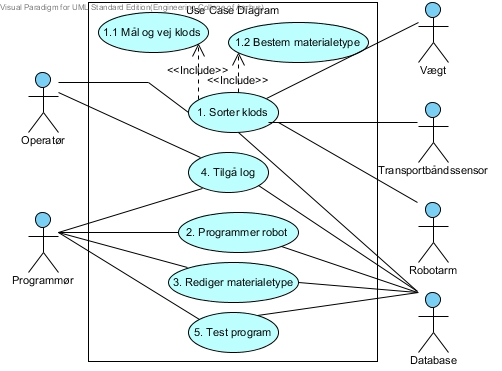
\includegraphics[scale = 0.7]{Diagrammer/Use_Case_Diagram.jpg}
\caption{Use Case diagram}
\label{fig:UseCaseDia}
\end{figure}

Som det fremg�r af Use Case diagrammet, figur 13,  er der to prim�re akt�rer, operat�ren og programm�ren, mens forskellige hardware (v�gt, robotarm og Transportb�ndssensor) og softwareenheder (database) indg�r som sekund�re akt�rer.
\\
Ligeledes kan det ses, at systemet har fem Use Cases. \textit{Use Case 1: Sorter Klods} er initialiseret af operat�ren, mens \textit{Use Case 2: Programmer robot, Use Case 3: Rediger materialetype} og \textit{Use Case 5: Test Program} er initialiseret af programm�ren. Det skal n�vnes at et af normalforl�bene i\textit{ Use Case 2: Programmer robot} ogs� kan initialiseres af operat�ren. \textit{Use Case 4: Tilg� log} kan b�de initialiseres af operat�ren og af programm�ren, da de begge kan have behov for at se, hvad sker i systemet. Include Use Casene til \textit{Use Case 1: Sorter klods} initieres gennem \textit{Use Case 1: Sorter klods}, da de blot er en hj�lp til at f� en klods sorteret.
\\\\
Alle Use Casene har en t�t relation til brugergr�nsefladen, og de fleste bliver initieret gennem denne, s� hvis det �nskes at se eksempler p� dette, henvises til \textit{afsnit 3.4 Gr�nseflader til eksterne softwareakt�rer}, hvor selve brugergr�nsefladen pr�senteres og beskrives.
\end{document}